\section{Introduction}

[TODO: Intention, hypotheses and results of the study]

Ethical, legal and social considerations are also part of my thesis.


Discussion centers on potential practical implications of the present results, as well as on prospects for future research.

\clearpage

\section{Background}

	\subsection{Motivation}
	
	E-learning providers are looking to improve the learning experience of their users and make progress as effective as possible. 
During a typical learning session each learner is subject to a range of volatile emotional states that help or hinder their learning success. 
Several factors and stimuli, both internal and external, can influence emotions. 
When we take this knowledge about emotions into account a new way to manage a learning session opens. We can incorporate this knowledge into learning sessions and provide a more appropriate task and interface for the learner.

The goal of the paper is to examine a relationship between the emotional aspect of a user interface in an e-learning system and its effect on the performance of the learner.


\begin{center}
	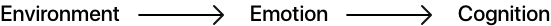
\includegraphics[width=200px]{graphics/relation1.png}
\end{center}
 
There is strong evidence of the surrounding environment having an influence on emotion \cite{Johnson2000, Arockiam2013, Bertamini2013}. This includes, for example, an e-learning system on the screen in front of the learner. In a similar fashion several studies have shown a correlation between emotion and cognition (Section \ref{sec:emotion-cognition}).

\begin{center}
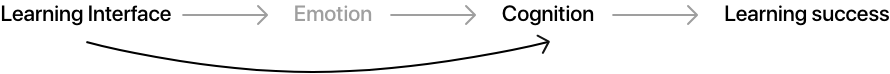
\includegraphics[width=300px]{graphics/relation2.png}
\end{center}

There is a logical argument of the existence of a transitive relation between these parameters, which could confirm the dependency of the edge variables. 
I.e. exposure to several interfaces each with a different emotional charge during an on-line lesson should lead to a difference in performance when working on the same task.
Insufficient research confirming this connection and explaining the effects has been published yet. 

In this paper I would like to explore to which extent the final parameter "learning success" can be influenced with the limited surface of contact that can be addressed through a learning interface on the screen.
	
		
	\subsection{Research basis} \label{sec:research}
	
	\toDo{about 10 pages of research}
	
	Information architecture and display types play an important role in learning comprehension, attention and learning success. \cite{McCrudden2017} describe the effects of different types of visual display on cognitive processing. They highlight the important aspects of visual guidelines, the basics of human understanding and  memory, as well a way to quantify those under processing efficiency. One of their conclusions is that "displays should be designed to support the selection of important information" \cite[p.633]{McCrudden2017}
	
	There is, however, a case to be made with respect to the same visual display that can be put forth in front of participants under differentiating emotional states. There is strong evidence that emotions play a role in information processing and, as a consequence, can have an effect on the resulting performance. Section \ref{sec:emotion-cognition} discusses closer existing research supporting a connection between emotion and cognition.
	
	Evidence also suggests that specific emotion can be caused through the use of emotional design features. Section \ref{sec:emotional-design-features} proposes a set of general rules for emotional design based on previous research.
	
	A recent study \cite{Haaranen2015} suggests that wrong choice of emotional design patterns can yield contra-productive results. It reports lover concentrations levels in the experiment group compared to control group using abstract graphics when learning object-oriented programming (OOP). Due to their choice of presentation and the topic of learning, the material has not been perceived as serious and lead to lower self-reported concentration levels.
		
		\subsubsection{Emotion theory} \label{sec:emotion-theory}
		
		To understand how emotion acts as a mediator to e-learning and learning in general it is important to see what emotion is and what causes it.
		
		From a biological perspective \textbf{emotion} is a collection of responses triggered from parts of the brain to the body or other parts of the brain. A series of such responses results in an \textit{emotional state} and is defined by changes within the body. \cite{Damasio1998}
	
		Emotion is caused by various internal and external events. Internal events can be immune activity or hormone changes. External events - observed or felt in the outside world - contribute additionally to internal ones. People have do direct access to the causal connections of emotions and little to no control of them. One can undergo a change of emotion without knowing why. \cite{Russell2003}
		
		Russell proposes that at the base of any emotion the experienced states are either good or bad, energized or enervated. As such these are the two "core affects" that govern our perception, behavior and cognition. \cite{Russell2003}. 
		
		There are individual differences of average levels of core affect and its responsiveness to stimuli due to the genetic differences. \cite{Russell2003}
		
		Over the years of psychological research, models of emotion have taken a range of representations. 
		A popular approach is the "Circumplex Model of Affect" \cite{Russell1980}, where emotions can be summarized and laid out in a two-dimensional space. The horizontal axis describing the "pleasure" (futher used as valence) dimension. The vertical axis - the arousal dimension. These dimensions are treated as independent.
		
		Assumptions in this paper are largely based upon the "Circumplex Model". I classify possible emotional states into four quadrants which are mutually discrete. To simplify, they are be labeled for further reference as shown in figure \ref{fig:valence_arousal_model}):
		\begin{enumerate}
			\item[Q1:] Angry 	(Quadrant 1)
			\item[Q2:] Happy 	(Quadrant 2)
			\item[Q3:] Sad 		(Quadrant 3)
			\item[Q4:] Relaxed 	(Quadrant 4)
		\end{enumerate}
		
		Some sources suggest a third dimension of "dominance" to be added to the representation to for the PAD (Pleasure, Arousal, Dominance) Model. Dominance dimension ranges from controlling and dominant to controlled/submissive. For example, fear and anger are very similar on a 2 pleasure and arousal scales. On the dominance scale anger is a dominant emotion, while fear is submissive. \cite{Mehrabian1974}
		This study does not consider the dominance dimension in the analysis framework. 
		
		\cite{Harley2016} Measuring Emotions: A Survey of Cutting Edge Methodologies Used in Computer-Based Learning Environment Research: An Emotion primer, use as source
		
		\begin{figure}
			\begin{center}
				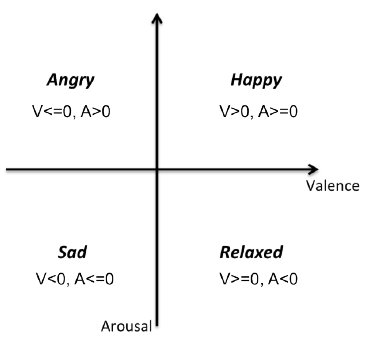
\includegraphics[width=150px]{graphics/Valence-Arousal-model-showing-the-quadrants-of-the-four-emotion-tags-used-in-this_W640.jpg}
				\caption{Valence Arousal Model. Figure from \cite{Song2013} \label{fig:valence_arousal_model}}
				
			\end{center}
		\end{figure}
		
		
		\toDo{[TODO]: summarize Valence-Arousal model and explain 4 groups}
		
		
		
		\subsubsection{Visual interface and emotion}
		
		\cite{Desmet2007} demonstrates in their research that physical objects can cause significant emotional response and that modifying design attributes can successfully contribute to creating of desired response.
		Both physical objects and digital visuals are, in essence, interfaces. As corroborated by emotion theory any interface we acknowledge and, especially interact with can cause an emotional response. 
		
		Nowadays, user's attention spans are increasingly short and distractions are more common than ever. With the advent of Web 2.0 and the increasing speed or computers and consumer oriented digital products we are accustomed to quick, precise responses. Users grant low tolerance to shortcomings in an interface. Abundance of alternatives leads to consumers choosing the product that can cause the most pleasant emotional affect.
		
 		Digital interfaces are extremely flexible to experimentation and modification at a relatively low cost, compared to conventional physical products.
 		The industry  experimentation, research, and improvements in user interface practices, especially when it comes to emotions.
		%%%%%%%%%%%%%%%%%%%%%
		
		
		%\paragraph{Literature review}
		
		A paper by L. Arockiam et al \cite{Arockiam2013} suggests that, based on previous research and their own findings, optimal user interface can be achieved when you add a person's personality traits into consideration. This finding could mean a mediating effect of participant preference on the universality of interface attributes aimed at evoking high arousal. 
		
		Current study aims to find a general set of attributes that should evoke high arousal and positive valence.
		
		\paragraph{Color}
		
		A 1996 research paper \cite{Pert1996} provides a wide overview of literature and delivers important insight about color, citing an array of previous research. The following paragraphs on color reference \cite{Pert1996}, unless otherwise stated. The paper provides a categorization of color effect on a person into three distinct types: physiological, psychological, and learning related. As asserted in \ref{sec:emotion-theory} and \ref{sec:emotion-cognition} all of these can be understood as interrelated, as both physiological and psychological processes take an effect on emotion and learning.
						
		Nevertheless, following the distinction made by Pert et al., a \textit{physiological effect}, in particular - arousal is shown in \cite{Wilson1966} with reported higher galvanic skin response (GSR) measurements for red color as opposed to green. 
		Nourse and Welsh (1971) reported higher GSR for violet than green.
		Jacobs and Hustmyer (1974) found that red was significantly more arousing than yellow or blue, 
		Jacobs and Suess (1975), although, found that red and yellow resulted in a higher anxiety state scores than blue or green.
		
		Overall \cite{Pert1996} suggests that spectral extremes, like red and violet, cause greater arousal than colors in the middle of the spectrum.
		
		Under \textit{psychological effects} of color Pert analyses preference, meaning and perceived harmony between colors.
		
		A 1941 study \cite{Eysenck1941} ranks preferences of colors presented on colored pieces of paper. 
		The order of preference is: 1 - blue, 2 - red, 3 - green, 4 - violet, 5 - orange, 6 - yellow. Earlier studies conducted among 21,060 subjects conclude the same average selection of color preference. Important trait of these results is that the order is observed to be the same for all races and for both men and women. A single difference is manifested at the far end of the preference scale, where men choose orange over yellow, while women choose yellow over orange.
		
		In 1963 \cite{burnham1963color} affirms the lack of significant differences between men and women or between different races on color preference.
		
		These findings are expanded in a study on color and emotion \cite{Valdez1994}, where the results show that men and women have a similar emotional reaction to variations in saturation and brightness. A slight consistently stronger emotional response is recorded by women compared than men. This could suggest that women are more influenced by visual stimuli.
		
		Schaie (1966) reports, somewhat contrary to previous findings, that color preferences relate to personality of an individual and can vary. A stronger preference of cooler colors by introverts and warmer colors by extroverts is reported by C. Robinson (1975).
		
		A study among school children between first and twelfth grade finds that girls of all ages prefer brighter colors as compared to boys (Child, et al., 1968). This finding is of limited relevance and may find limited degree of comparability to adults, as it focuses on children. Winn and Everett (1979) states that color in pictures has greater impact on meaning among young people.
				
		In a study by Adams and Osgood in 1973 conducted across 23 different cultures a general preference for cool colors (blue/green) compared to warm colors (red/yellow) has been established. Pert asserts that cool colors tend to rate higher on average across cultures, ages and individual characteristics.
		
		Among the suggested uses of color Pert suggests using a color like "highly saturated red and violet to attract attention and to create an emotional response" \cite{Pert1996}, and to consider color associated meanings i.e. red means stop, the meanings attributed to colors can also differentiate among cultures.
		
%		An extensive study on effects of hue, saturation and brightness of color of emotional 
		
		While colors at the ends of the spectrum cause greater arousal, those in the middle of the spectrum, like green and cyan, are reported to be best for emphasis. \cite{Pert1996}. The paper suggests that red, having an arousal effect could potentially be more effective than middle-spectrum colors to attract and hold attention. Brightness of color is suggested to affect the mood attributed to that color more than it's hue.

		
		A 1994 study of effect of color on emotions completed two studies. The first study with two hundred and fifty subjects analyzed emotional impact of color saturation and brightness. Emotions are specified on three scales: arousal, pleasure and dominance.
		 had 121 people rate different hue found that hue \cite{Valdez1994}
		
		
		\cite{Wilms2018} Color and emotion: effects of hue, saturation, and brightness
		
		\paragraph{Color and learning} Color use in a learning and cognition setting is approached in the following studies.
		
		(Kanner and Rosenstein, 1960) studies color-effectiveness at Fort Monmouth in typical army training procedure. 11 video lessons are used with monochrome and colored versions of television. No significant differences are found in learning between both \cite{Pert1996}. Historical context is important here, as at this time television resolution and color reproduction has not been as vivid and realistic as nowadays, as stronger, more saturated colors are found to be more potent in causing emotional affect \cite{Valdez1994}
		
		(so far black and white and color has not yielded any significant difference in learning)
		In education "colored materials are preferred by learners." \cite[p.25]{Pert1996}
		
		1972: those who viewed colored transparencies had had a more positive attitude toward transparencies than \cite{Pert1996}
		
		In a research study on color coding, Lamberski and Dwyer (1983) concluded that color is an attention-getting device that can provide measurable effects on learning that cannot be accounted for by words and labels. \cite{Pert1996}
		
		Search Tasks: 
		gain in efficiency, indicated by decreased search time, with codes of up to five colors \cite{Pert1996}
		
		Color was found to be useful in grouping information
		
		color versions resulted in higher recognition- memory scores (immediate recognition memory test)\cite{Pert1996}
		
		as the variable of visual complexity increases, so does the degree of recall. (Berry (1991a)) \cite{Pert1996}
		
		The key factor relating to color and cognitive learning seems to be that it is of value when it emphasizes relevant cues, is used as a coding device, or when it is a part of the content to be learned (Dwyer and Lamberski, 1982- 83; Levie, 1973; Pruisner, 1993; Wedell \& Alden, 1973). \cite{Pert1996}
		
		\textbf{Non-objective Measures}
		
		(Scanlon, 1970). Scanlon suggests that the color versions (Grey Cup football game) create emotional effects that detract from attention to details.
		
		
		Random use of color is not generally associ- ated with increased learning. There is some evidence that color can increase retention. This \cite{Pert1996}

		
		Good sources:
		
		\cite{Valdez1994} - effects of color on emotions
		
		\cite{Plass2014} - Emotional design in multimedia learning: Effects of shape and color on affect and learning
		
		\cite{Swasty2017} - Does Color Matter on Web User Interface Design?
		
		\cite{Pert1996} - Color Research and Its Application to the Design of Instructional Materials
		
		\cite{Tekirdag2015} - The Effect of Colour on Human Body and Psychology
		
		\paragraph{Shapes}
		
		\paragraph{Emoticons / Emojis} Emoticons
		
		\cite{Dunlap2016} - What Sunshine Is to Flowers: A Literature Review on the Use of Emoticons to Support Online Learning
		
		\cite{Walther2001} when analyzing the "Impacts of Emoticons on Message Interpretation in Computer-Mediated Communication" observed that for positive messaging positive emoticon (textual representation) improves happiness perception rating for that message. 
			
		%%%%%%%%%%%%%%%%%
		
		\subsubsection{Emotion and cognition} \label{sec:emotion-cognition}
		
		Emotion has a strong impact on cognitive processing \cite{Sakaki2012}
		
		A 2004 cognitive neuroscience study \cite{Dolcos2004} scanned participants brain activity, while rating emotional pictures. The study makes several relevant conclusions. First, that different parts of the brain show stronger activity when exposed to positive compared to negative stimuli. Second, that high arousal stimuli lead to greater successful encoding activity, or in other words - rate of recall, than neutral stimuli. 
		
		In other words, brain response is different for arousing stimuli of positive valence compared to negative valence. Furthermore memory is mediated, in part by both - valence and arousal levels. It provides basis to the assumption that variation on both dimensions is necessary to adequately reflect effects within e-learning context. Study design in \ref{sec:study-design} depends heavily on this assumption.
		
		\cite{Bradley1992} Remembering pictures: Pleasure and arousal in memory.
		 Pictures rated as highly arousing were remembered better than low-arousal stimuli.
		
		\cite{Sternberg2010} Emotion and E-Learning
		
		\cite{Leutner2014} Motivation and emotion as mediators in multimedia learning
		
		\cite{Lee2014} The effects of various multimedia instructional materials on students’ learning responses and outcomes: A comparative experimental study
		
		\cite{Heidig2015} Emotional design in multimedia learning: Differentiation on relevant design features and their effects on emotions and learning
		
		\cite{Plass2016} Because working memory can only hold a limited amount of information (Baddeley, 1986, Cowan, 2001), processing of multimedia information is performed under these memory constraints
		
		\cite{Chung2015} Emotion and multimedia learning: an investigation of the effects of valence and arousal on different modalities in an instructional animation (The results showed that both arousing groups outperformed calm groups on a recall test only in the written-text group regardless of valence, while emotional valence and arousal did not significantly influence learning performance in the spoken-text group. The results provide partial support for the LC4MP model and imply that the arousing emotional state has the potential to enhance multimedia learning.)
		
		\cite{Thompson2001} AROUSAL, MOOD, AND THE MOZART EFFECT
		
		\paragraph{Emotional design and Learning} 
		
		\cite{Plass2014} Emotional design in multimedia learning: Effects of shape and color on affect and learning
		
		\cite{Mayer2014} Benefits of emotional design in multimedia instruction
		For the enhanced group, the graphics were redrawn to render the host cell as a red face with expressive eyes (registering surprise, fear, and sickness at various stages in the process), and the virus as a blue face with fierce eyes and with a green dot at the end of each of the blue tentacles surrounding the virus face. The enhanced group performed better than the control group on a subsequent learning test
		
		\cite{Le2018} Heart rate variability reflects the effects of emotional design principle on mental effort in multimedia learning
		
		\cite{Plass2016}
		
		\cite{Chang2014} Effects of seductive details evidenced by gaze duration.
		(Lehman et al., 2007) showed that the presence of sentences with seductive details had a significant
		negative effect on the amount of time the participants spent. According to the recall analysis, those
		participants who read the baseline passage (i.e., no seductive
		sentences) were significantly more likely to recall important information than those who read the seductive passage
		reading baseline sentences.
		
		\cite{Le2018} Heart rate variability reflects the effects of emotional design principle on mental effort in multimedia learning
		
		The effect of emotional design on mental effort investment was investigated
		Results validate incorporating positive emotion graphics in multimedia instructions.
		Stronger decrease of HF HRV were observed in positive design group.
		
		\cite{Brom2018} How effective is emotional design? A meta-analysis on facial anthropomorphisms and pleasant colors during multimedia learning.
		
		Anthropomorphisms and pleasant colors should enhance multimedia learning
		Anthropomorphisms/colors consistently increased learning outcomes
		Their effects on affective-motivational states were weaker and less robust.
		Anthropomorphisms/colors are beneficial, but the mechanism is unclear.
		\cite{Lee2014}
		
		\cite{Uzun2018} Exploring the effect of using different levels of emotional design features in multimedia science learning
		
		
	
	\subsection{Hypotheses}
	
		To validate if there is a difference between emotional responses to the two different design approaches and consequently check if these differences lead to a different performance of learning sessions two hypotheses are proposed:
	
		\paragraph{Hypothesis 1.} H$_{0}$: Two different proposed interfaces do not result in a significant difference in emotional response.
		
		\paragraph{Hypothesis 2.} H$_{0}$: Performance of participants on memory and creativity tasks, as measured by selected study design parameters, during the experiment is equal using interface 1 compared to using interface 0.

\section{Approach and Methods}

To facilitate the study I make assumptions about the medium in which e-learning is usually conducted. Based on previous research (\ref{sec:research}) I define study design parameters and a set of target variables that are measured and evaluated.

	\subsection{Medium}
	
	The study is to be conducted online under a "real-life" scenario. This means, that the experiment is to be run in a browser-capable web-application runnable on modern personal computers. Like most e-learning software the  application used in the study is browser-based and usually used in a user's home or public venue.
	
	\subsection{Study design} \label{sec:study-design}
	
	Goal of the current study is to determine emotional response difference to provided emotional design implementation (Interface 1) compared to the control group that is provided with a stricter desaturated design (Interface 0). Differences include use of color, shapes, language, font style, interaction responsiveness, animation. The similarities or - constant variables - across both interfaces include any accessibility features and general usability heuristics, such as contrast ratio level, size and placement of elements on a screen. Further details of the emotional design aspects, that are included in the current implementation are shown in section \ref{sec:emotional-design-features}
	
	Participants of the study are not informed about the existence of another interface as a variable but rather only made aware about being emotionally influenced by preconditioning and that their performance during the experiment is being measured. Abundance of timers throughout the test highlight the time sensitivity of the tasks to the participant. This is a \textit{between-subject} experiment with each combination of four preconditioning and two interface version is tested once for each participant
	
	The experiment can be outlined and split into following steps:
	
	\begin{enumerate}
		
		\item[0.] \textbf{Clustering:} Each participant is assigned an interface version (one of two) and the preconditioning group (one of four) at random before first load of the application.
		
		\item \textbf{Emotional report:} A short emotional self-reporting questionnaire (SAM \ref{sec:selfeval}) is used to acquire initial valence and arousal ratings
		
		\item \textbf{Preconditioning:} Each participant is shown a set of emotional images and preconditioned to be in one of 4 states:
			\textbf{1}: Positive valence / high arousal;
			\textbf{2}: Negative valence / high arousal;
			\textbf{3}: Positive valence / low arousal;
			\textbf{4}: Negative valence / low arousal;
			
		Choice of stimuli and their presentation is described further in chapter \ref{sec:preconditioning}
			
		\item \textbf{Emotional report:} Emotional self-reporting questionnaire (SAM \ref{sec:selfeval}) to validate, whether preconditioning has had a sufficient and expected effect on the participant.
		
		\item \textbf{Experiment 1:} Slightly modified classic memory game. The participant is presented with a grid of tiles, each tile containing an image. During 10 seconds at the beginning of the experiment all tiles are open to allow to memorize the images. After which all images are hidden. Only 2 tiles can be opened at any one time. Once both tiles of the same image are open they are marked as solved. The goal is to solve all tiles. Detailed description in section \ref{sec:memory}
		
		\item \textbf{Experiment 2:} Remote Associates Test (RAT). A generalized creativity test developed by Mednick \cite{Mednick1962} in 1962. Each participant is presented with a number of word sets. Each set consists of 3 words that are shown to the participant and one target word that is hidden from the them. The target word is semantically connected to all 3 visible words. Detailed description in section \ref{sec:creativity}
		
		\item \textbf{Emotional report:} A second emotional self-reporting questionnaire (SAM \ref{sec:selfeval}) is used to establish, whether and which effect tasks and interface have had on the participant's emotion.
		
		\item \textbf{Demographic data:} Final step adds additional personal context data for each participant through a questionnaire to complement data analysis (discussed in \ref{sec:demographics}).
		
	\end{enumerate}
	
	\subsection{Preconditioning sequences} \label{sec:preconditioning}
	
	\paragraph{Finding a preconditioning sequence}
To facilitate emotional conditioning I selected a specialized sequence containing images with a corresponding emotional charge.
Each sequence contains 21 to 39 \todo{more precise} images with each displayed for about 5 seconds.

Each subject is assigned one of four preconditioning sequences. Each sequence is aimed to condition the subject into one of the 4 quadrants, described though a valence-arousal emotional model. To simplify we will label (\ref{fig:valence_arousal_model}) them as:
\begin{enumerate}
	\item Angry (Quadrant 1)
	\item Happy (Quadrant 2)
	\item Sad (Quadrant 3)
	\item Relaxed (Quadrant 4)
\end{enumerate}


\begin{figure}
\begin{center}
	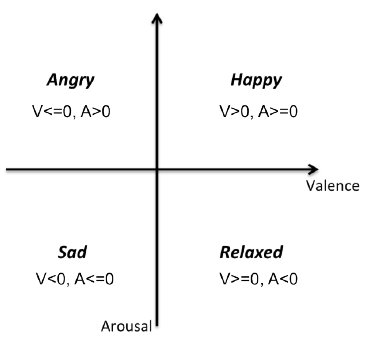
\includegraphics[width=150px]{graphics/Valence-Arousal-model-showing-the-quadrants-of-the-four-emotion-tags-used-in-this_W640.jpg}
	\caption{Valence Arousal Model \cite{Song2013} \label{fig:valence_arousal_model}}
	
\end{center}
\end{figure}

There are several emotional image data-sets available for academic purposes such as GAPED \cite{Dan-Glauser2011}, OASIS \cite{Kurdi2017}, IAPS \cite{Lang1997} and NAPS \cite{Marchewka2014}. While NAPS is offering the highest realism and quality of images, the range images seems to cover "sad" and "happy" to a less pronounced degree. In general, strong negative valence values are accompanied with high arousal values across all analyzed data-sets. Causing sadness is a challenging task. In current preconditioning sequences I am using the \textbf{OASIS} database. It has relatively wide spread of emotions compared to other sets.

Keeping in mind the need for a clear separation between groups in terms of their emotional state into account, I limited emotional images to moderately strong stimuli values, thus avoiding extreme reactions and unrealistic emotional states. It can be assumed that in most cases, people who attend e-learning lessons will have moderate levels of emotional charge. It is important to note that quadrant 1 - angry and quadrant 2 - happy has a more pronounced representation in emotional databases due to an easier and more prevalent stimuli availability. As such quadrant 1 and quadrant 2 have stronger stimuli compared to quadrant 3 and 4. It is expected that there will be a significant difference between emotion ratings of participants across these groups.

It is understood that the e-learning interface under real conditions will only cause mild-to-moderate changes to a mood.


\begin{figure}
	\centering
	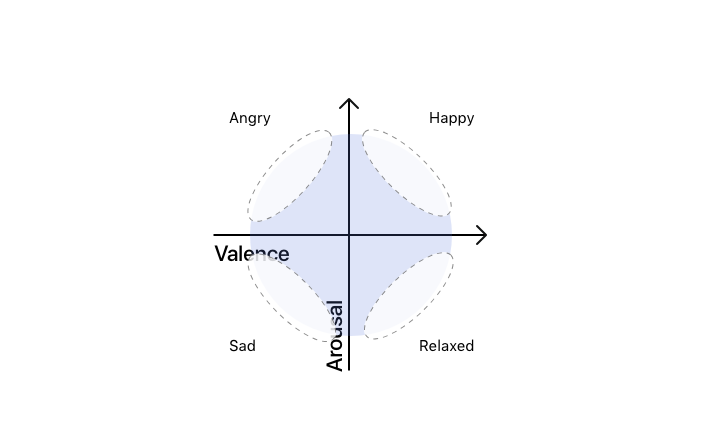
\includegraphics[width=0.7\linewidth]{graphics/Valence-Arousal-Model-1.png}
	\caption{Focus levels of emotional states on valence arousal model}
	\label{fig:valence-arousal-model-2}
\end{figure}

Illustration \ref{fig:valence-arousal-model-2} highlights with dashed outline areas the target arousal and valence values

	
	\subsection{Emotional Design Features} \label{sec:emotional-design-features}

	Studies shown in section \ref{sec:research} strongly suggest a connection between user interface and learning performance. They analyze performance and presentation based on concrete learning content examples. In present study I attempt to generalize the findings to a more universal set of guidelines that is not specific to certain content and could be applied to any e-learning topic.
	
	Emotional design has a limited surface area of possible modifications due to the focus being on the content. Under real conditions it can be expected that the e-learning interface will cause mild-to-moderate changes to affect. In part, those changes are also attributed to the task at hand, rather than the emotional design attributes.
	
	\cite{Brom2018}: Anthropomorphisms/colors consistently increased learning outcomes.
	
	\cite{Le2018}: Compared to the participants in the neutral design group, the participants in the positive emotional design group performed better on a subsequent retention test
	
	\cite{Uzun2018} Exploring the effect of using different levels of emotional design features in multimedia science learning


	\clearpage

\paragraph{Developing a high performing interface}

There is a multitude of studies that analyze user interface design and user emotion. In following I will summarize them in respect to UI features tailored towards high performance

\paragraph{Literature review}

A paper by L. Arockiam et al \cite{Arockiam2013} describes that, based on previous research and their own findings optimal ui can be achieved based on a person's personality traits. We will limit ourselves to a universal set of changes that should evoke high arousal, positive valence and therefore have an effect on learning outcome, rather than look for their preference. Nevertheless it is worth mentioning...

Color - PHYSIOLOGICAL

Wilson (1966) reported higher GSR measurements for red as opposed to green, and Nourse and Welsh (1971) reported higher GSR readings for violet than green. Using 24 male college students as subjects and saturated samples of red, yellow, green, and blue as stimulus materials, Jacobs and Hustmyer (1974) found that red was significantly more arousing than either yellow or blue, and green more than blue. Using 40 undergraduate students as subjects, Jacobs and Suess (1975) found that red and yellow resulted in higher anxiety state scores than blue or green when measured by the StateTrait Anxiety Inventory. Bloomer (1976) also reported that red increases heart rate. There appears to be some evidence that spectral extremes, especially red, cause greater arousal than mid-spectral colors. This may relate to the fact that wavelengths at the extremes of the spectrum, such as red and violet, focus at different points in the eye than wavelengths at the middle of the spectrum. \cite{Pert1996}

Color - PSYCHOLOGICAL

The selected order of preference was: (1) blue, (2) red, (3) green, (4) violet, (5) orange, (6) yellow. This selection agreed with the average rankings of color preference among 21,060 subjects reported in earlier investigations. The order was the same for all races and for men and women with one exception. Men chose orange over yellow whereas women chose yellow over orange. \cite{Pert1996}

no significant differ- ences between men and women or between subjects of different races.\cite{Pert1996}

girls of all ages preferred higher value, brighter, colors as compared to boys (Child, et al., 1968) \cite{Pert1996} (study among school age children from 1 to 12 grade)

Results on the evaluation scale supported the general preference for cool colors(bl~e and green) as compared with warm colors(red and yellow) and agree with previous findings by Adams and Osgood (1973) that red is a potent color while gray and black have low potency. \cite{Pert1996}

In a color-effectiveness study conducted at Fort Monmouth, typical army training procedures were used with 11 different television lessons (Kanner and Rosenstein, 1960). No significant
differences were found in learning between
monochrome and colored versions \cite{Pert1996}

Schaie (1966) pointed out that color prefer-
ences vary from individual to individual and relate to personality. \cite{Pert1996}

(so far black and white and color has not yielded any significant difference in learning) but "colored mate- rials are preferred by learners." \cite{Pert1996}

1972: those who viewed colored transparencies had had a more positive attitude toward transparencies than \cite{Pert1996}

In a research study on color coding, Lamberski and Dwyer (1983) concluded that color is an attention-getting device that can provide measurable effects on learning that cannot be accounted for by words and labels. \cite{Pert1996}

Search Tasks: 
gain in efficiency, indicated by decreased search time, with codes of up to five colors \cite{Pert1996}

Color was found to be useful in grouping information

color versions resulted in higher recognition- memory scores (immediate recognition memory test)\cite{Pert1996}

as the variable of visual complexity increases, so does the degree of recall. (Berry (1991a)) \cite{Pert1996}

The key factor relating to color and cogni-
tive learning seems to be that it is of value when it emphasizes relevant cues, is used as a coding device, or when it is a part of the con- tent to be learned (Dwyer and Lamberski, 1982- 83; Levie, 1973; Pruisner, 1993; Wedell \& Alden, 1973). \cite{Pert1996}

Non-objective Measures

(Scanlon, 1970). Scanlon suggests that the color versions (Grey Cup football game) create emotional effects that detract from attention to details.







Colors at the ends of the spectrum, red and
violet, seem to result in greater arousal, and
colors in the middle of the spectrum, yellow,
green, cyan, seem to be best for discriminating
detail. \cite{Pert1996}
	
	\subsubsection{Developing a high performing interface}
	
	\toDo{write which interface elements are considered}
	
	\begin{itemize}
		\item Roundness of shapes vs corners
		\item warm colors vs cold colors
		\item smiling faces vs "X"
		\item responsiveness of ui (hover states and movements)
		\item more animations (for spacial more realistic feeling) such as tiles
		\item font family (rounded and edgy)
		\item use of wording, tone of voice and language \cite{Hancock2007}
	\end{itemize}

	Memory experiment page shows a smiling face icon. On-site questionnaire is conducted during creation of the experiment to determine an icon which is portraying the strongest "happiness" emotion. A previous iteration also contained a female version of the image. It has been excluded to avoid an effect of gender bias.
	
	\begin{figure}
		\centering
		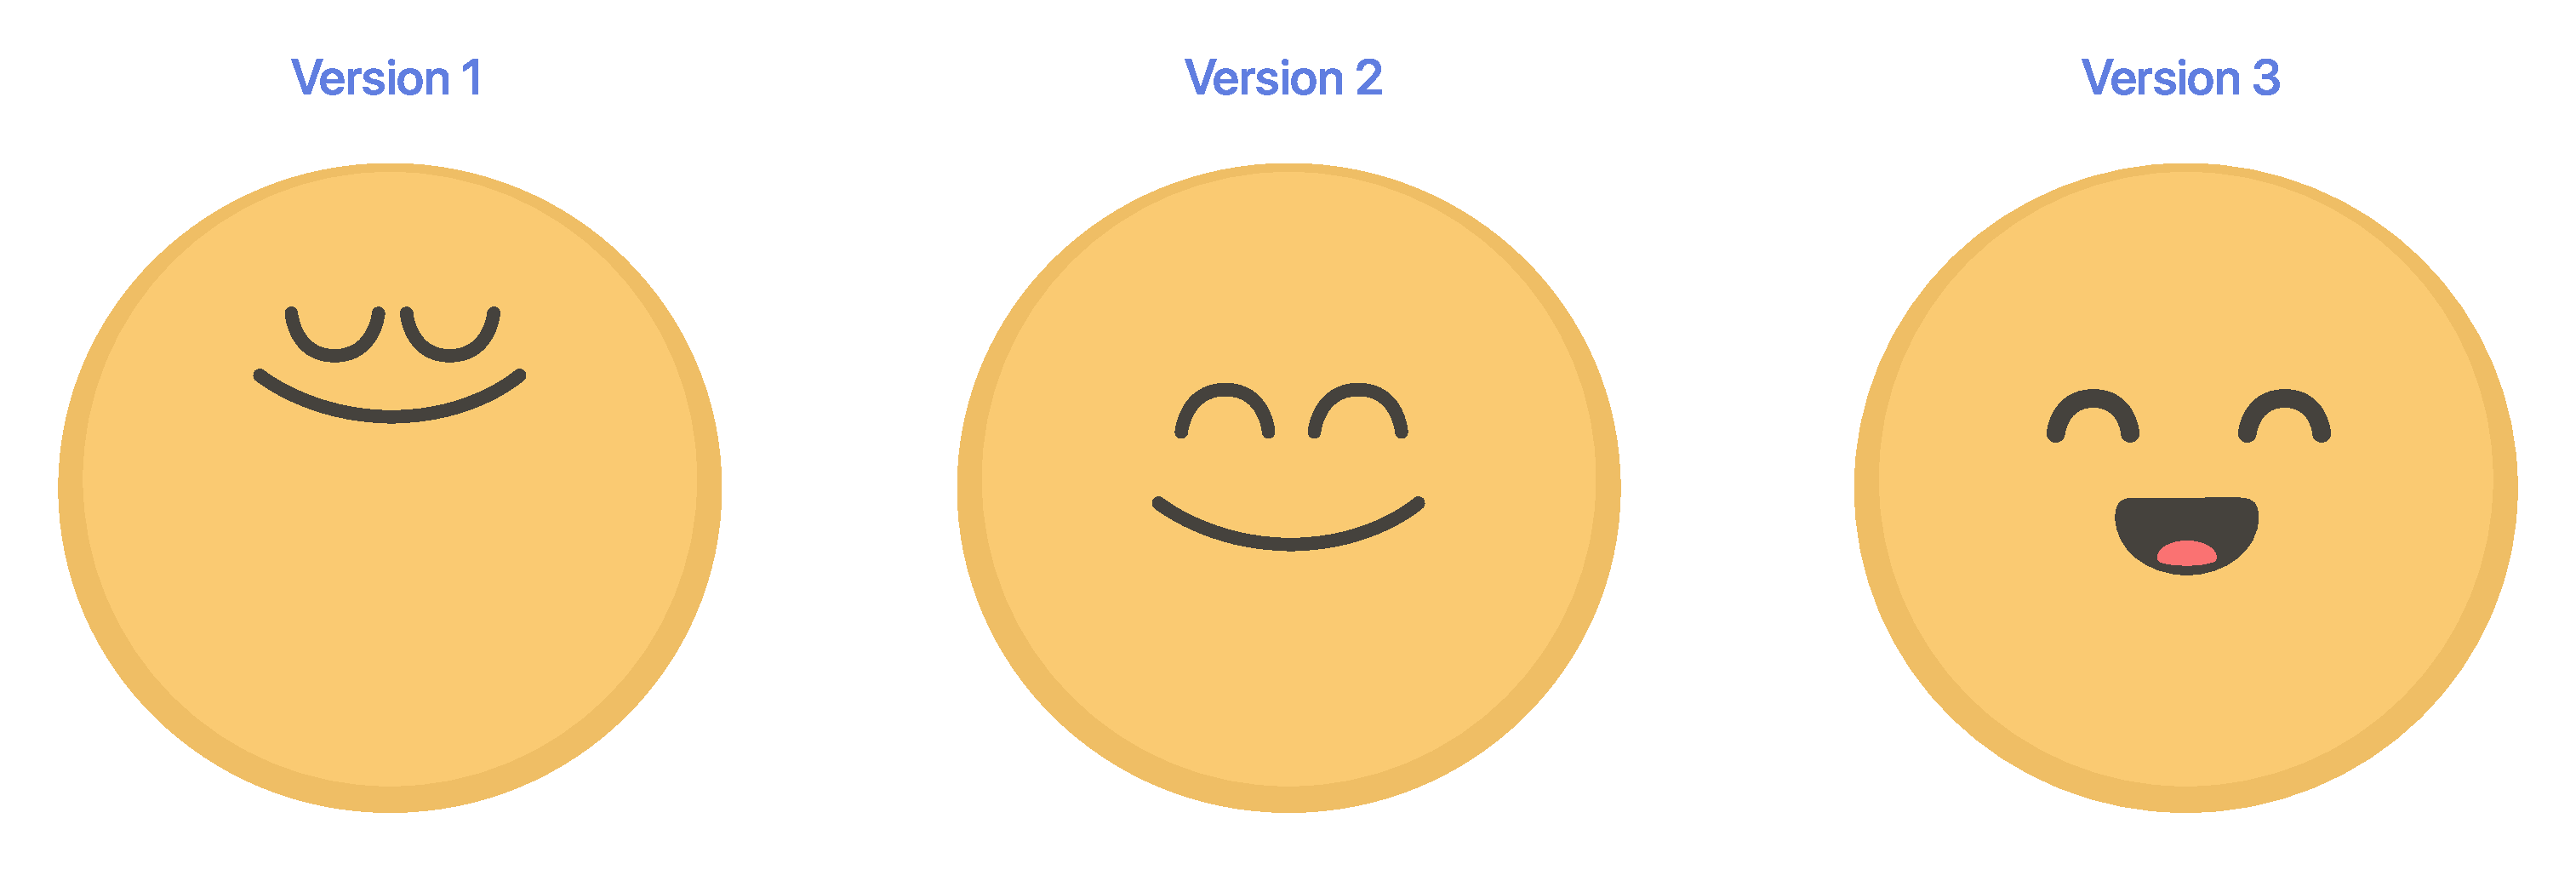
\includegraphics[width=0.7\linewidth]{graphics/smiling-icons}
		\caption{Choice of smiling face icons}
		\label{fig:smiling-icons}
	\end{figure}
	

	\cite{Zorko2017} The impact of the text and background color on the screen reading experience
	
	\clearpage
	\subsection{Experiments}

		\subsubsection{Experiment 1: Short term Memory} \label{sec:memory}
		
		The current memory experiment is based on a commercial "Memory" (TM) game developed in 1966, which has since been widely adopted in digital version on many platforms. 
		In this test participant attempts to match pairs of images which are displayed face down. 
		The constraint is that no more than two images can be turned around at any point in time. Subject begin turning cards at random order until they notice a second card that displays an image that has been turned over before. Once a pair of same images is found they are removed from the game.
		
		In the current study an adaptation of this game consists of \textit{twenty one pairs} of images that are arranged on a card grid of six by seven cards. Images for the cards in this experiment are taken from the Bank Of
		Standardized Stimuli (BOSS). BOSS is a set of normative visual stimuli intended for use in cognitive research. library \cite{Brodeur2010}. Images are taken in "png" format with a transparent background and placed on slightly colored card background in the interface. Both living and non-living images are selected. Among them are pictures of fruits and vegetables, technology items, and sport activity items.
		Table (\ref{table:boss-words}) presents the full list of the used BOSS image items in the current study.
		
		Women better \cite{McBurney1997}
		
		
		
		\paragraph{Experiment details}
		
		At the beginning of the game the participant is informed that they will see images for ten seconds an need to remember their locations. All images are shown open at the start as a measure to avoid random card selection at the beginning of the game, to allow the participant to identify and get familiar with the image range and selection.
		
		After ten seconds all images turn and the user sees the back-face of the cards in their respective design depending on the theme version.
		
		
		
		No practice run is provided in the memory experiment, as it is assumed that the interface and the mechanics of the game are readily familiar to the user \toDo{come back to this assumption in data discovery part}
		
		\paragraph{Activity logging}
		
		\textit{Experiment 1} activity is specified based upon generalized logging of activity in e-learning described in \ref{sec:activitylog}. Activity is logged with two types of actions: events and clicks. They are emitted when each of these conditions are met:
		
		\begin{itemize}
			\item Event: open positions for memorizing
			\item Event: close positions and start game
			\item Event: correct card pair opening
			\item Event: incorrect card pair opening
			\item Click on card one
			\item Click on card two
			\item Click on card when it is inactive
			\item Memory experiment finished
		\end{itemize}
		
		Card events contain location of the card in the grid, name of image and system context information.
		
		\paragraph{Performance variables:} \label{sec:memory-parameters} Participants \textit{memory performance} is defined by the total number of times any card is turned over. This measure goes in line with the memory test score employed by \cite{McBurney1997}
		
		Additionally, some secondary performance measures are defined as follows:
		
		\begin{itemize}
			\item total time taken to solve the test
			\item amount of cards opened before first incorrect match
			\item amount of card opens per minute - as a symbolic measure of haste, that could potentially correlate with arousal reports of the users.
			\item amount of incorrect pair openings - calculated by subtracting 42 from the main performance measure
		\end{itemize}
		
		\subsubsection{Experiment 2: Creative thought} \label{sec:creativity}
		
		A generalized creativity test developed by Mednick \cite{Mednick1962} in 1962 requires the participant to perform creatively. They are "asked to form associative elements into new combinations by providing mediating connective links" \cite[p. 226]{Mednick1962}. This test is called Remote Associates Test or RAT.
		It is developed in such a way that completing it does not require prior knowledge of any particular subject. 
		
		Participants are shown a set of three stimulus words from mutually remote associative clusters. Their task is to provide the mediating link between them. The link must be of an associative manner, rather than one that applies additional logic or inferences. Figure \ref{fig:exampleratset} shows an example of such word-set with a solution.
		
		A possible limitation on the universality of the test is knowledge of language and some cultural influence. Mednick himself states that RAT problems rely on "verbal associative habits could reasonably be assumed to be familiar to almost all individuals that have been brought up in this (USA) culture". The originally presented 30-element list of problems can have a certain degree of dependency on the cultural linguistic habits. For present study additional steps are taken to exclude possible problems due to these effects. 
		
		To minimize the limitation of language knowledge participant is required at the beginning of the study to comply with conditions, which contain (among others) "advanced English knowledge" (Appendix \ref{itm:participation_requirements}). After the tests the participants are asked to state whether or not they are native English speakers and to confirm their English knowledge level.
		
		\begin{figure}[h]
			\centering
			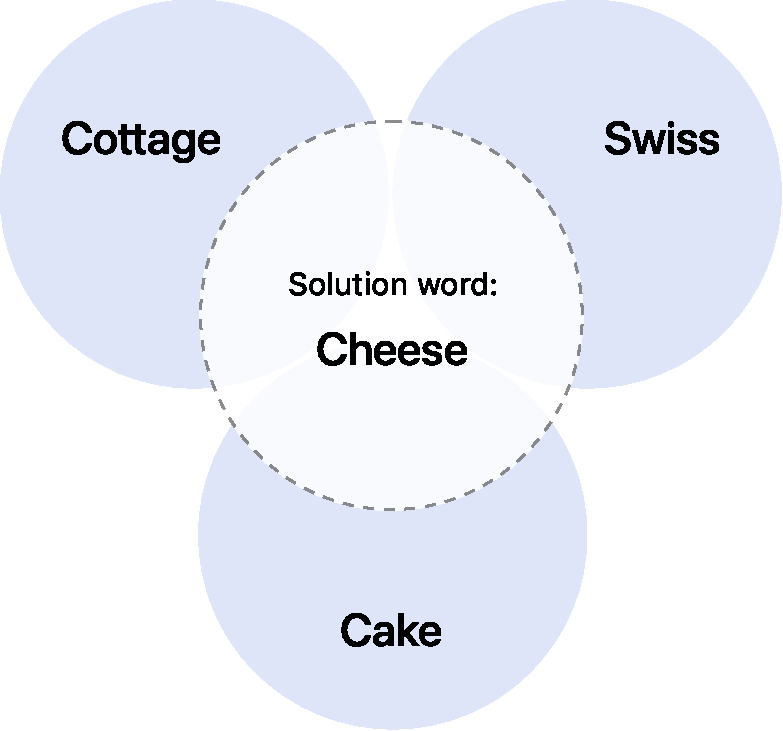
\includegraphics[height=0.3\textheight]{graphics/Example-RAT-Set}
			\caption{Example remote associate word-set 'Cottage, Swiss, Cake'}
			\label{fig:exampleratset}
		\end{figure}

		The current experiment uses a further development of the original Mednick's remote associate test presented by Bowden in a 2003 paper. Bowden et al. \cite{Bowden} have developed 144 sets of remote associate problems with an additional constraint. The solution word has to not only be related to the triad of stimulus words but additionally each of them should form a commonly used compound word or two-word phrase with the solution word. The solution word can build either the first part or the second part of the phrase.
		
		Bowden's word-sets are a subset of all possible remote associate problems and have been alternatively described as "compound word problems".
		
		\toDo{OPTIONAL: longer description of what Bowden proposes with some quotes}
		
 		I select \textbf{twenty} word-sets of a set of 144 compound remote associate sets that are proposed by \cite{Bowden}. Some of the easier (highest solving percentage rate among the 30-second threshold test participants, as provided by Bowden) word-sets are selected for present experiment. Additional filtering is applied to avoid colloquialisms and words that can be regarded as a local expression. As a result, the twenty word-sets should be challenging although solvable to a wide array of people from different backgrounds. Having very limited time and amount of words due to the experiment design, I attempt to maximize solution rates. Once the time to solve a problem runs out the problem is marked as unsolved for this participant session. Without a high degree of solved problems it gets more difficult to compare results.
		One of the indicators for performance is the time taken to solve a problem. (\ref{sec:creativity-parameters}).
 		
 		Table \ref{table:selected-remote-associates} presents the full list of the used RAT items in the current study. 
		
		\paragraph{Experiment details}
		
		Before the experiment begins, the participant is informed about the rules and what is expected from them with an introductory text:
		
		\begin{displayquote}
			"You will see three stimulus words. Attempt to generate a fourth word that is related to each stimulus word. When combined with each of the stimulus words will build a word pair that is a common compound word or phrase. The goal is to find a solution as fast a possible
			
			After 30 seconds you will see 2 words appearing as hints on the screen, only one solution is correct.
			The first 3 are practice sets and will allow you to train. During practice we will give you a hint after 10 seconds"
		\end{displayquote}
	
		The participant is shown three practice tasks which allow them to get used to the interface and the dynamics of the task. As most of the participants are remote and unsupervised it is important to give an intuitive set of instructions and avoid any confusion or variation due to unclear interface or task.
		
		\begin{figure}[h]
			\centering
			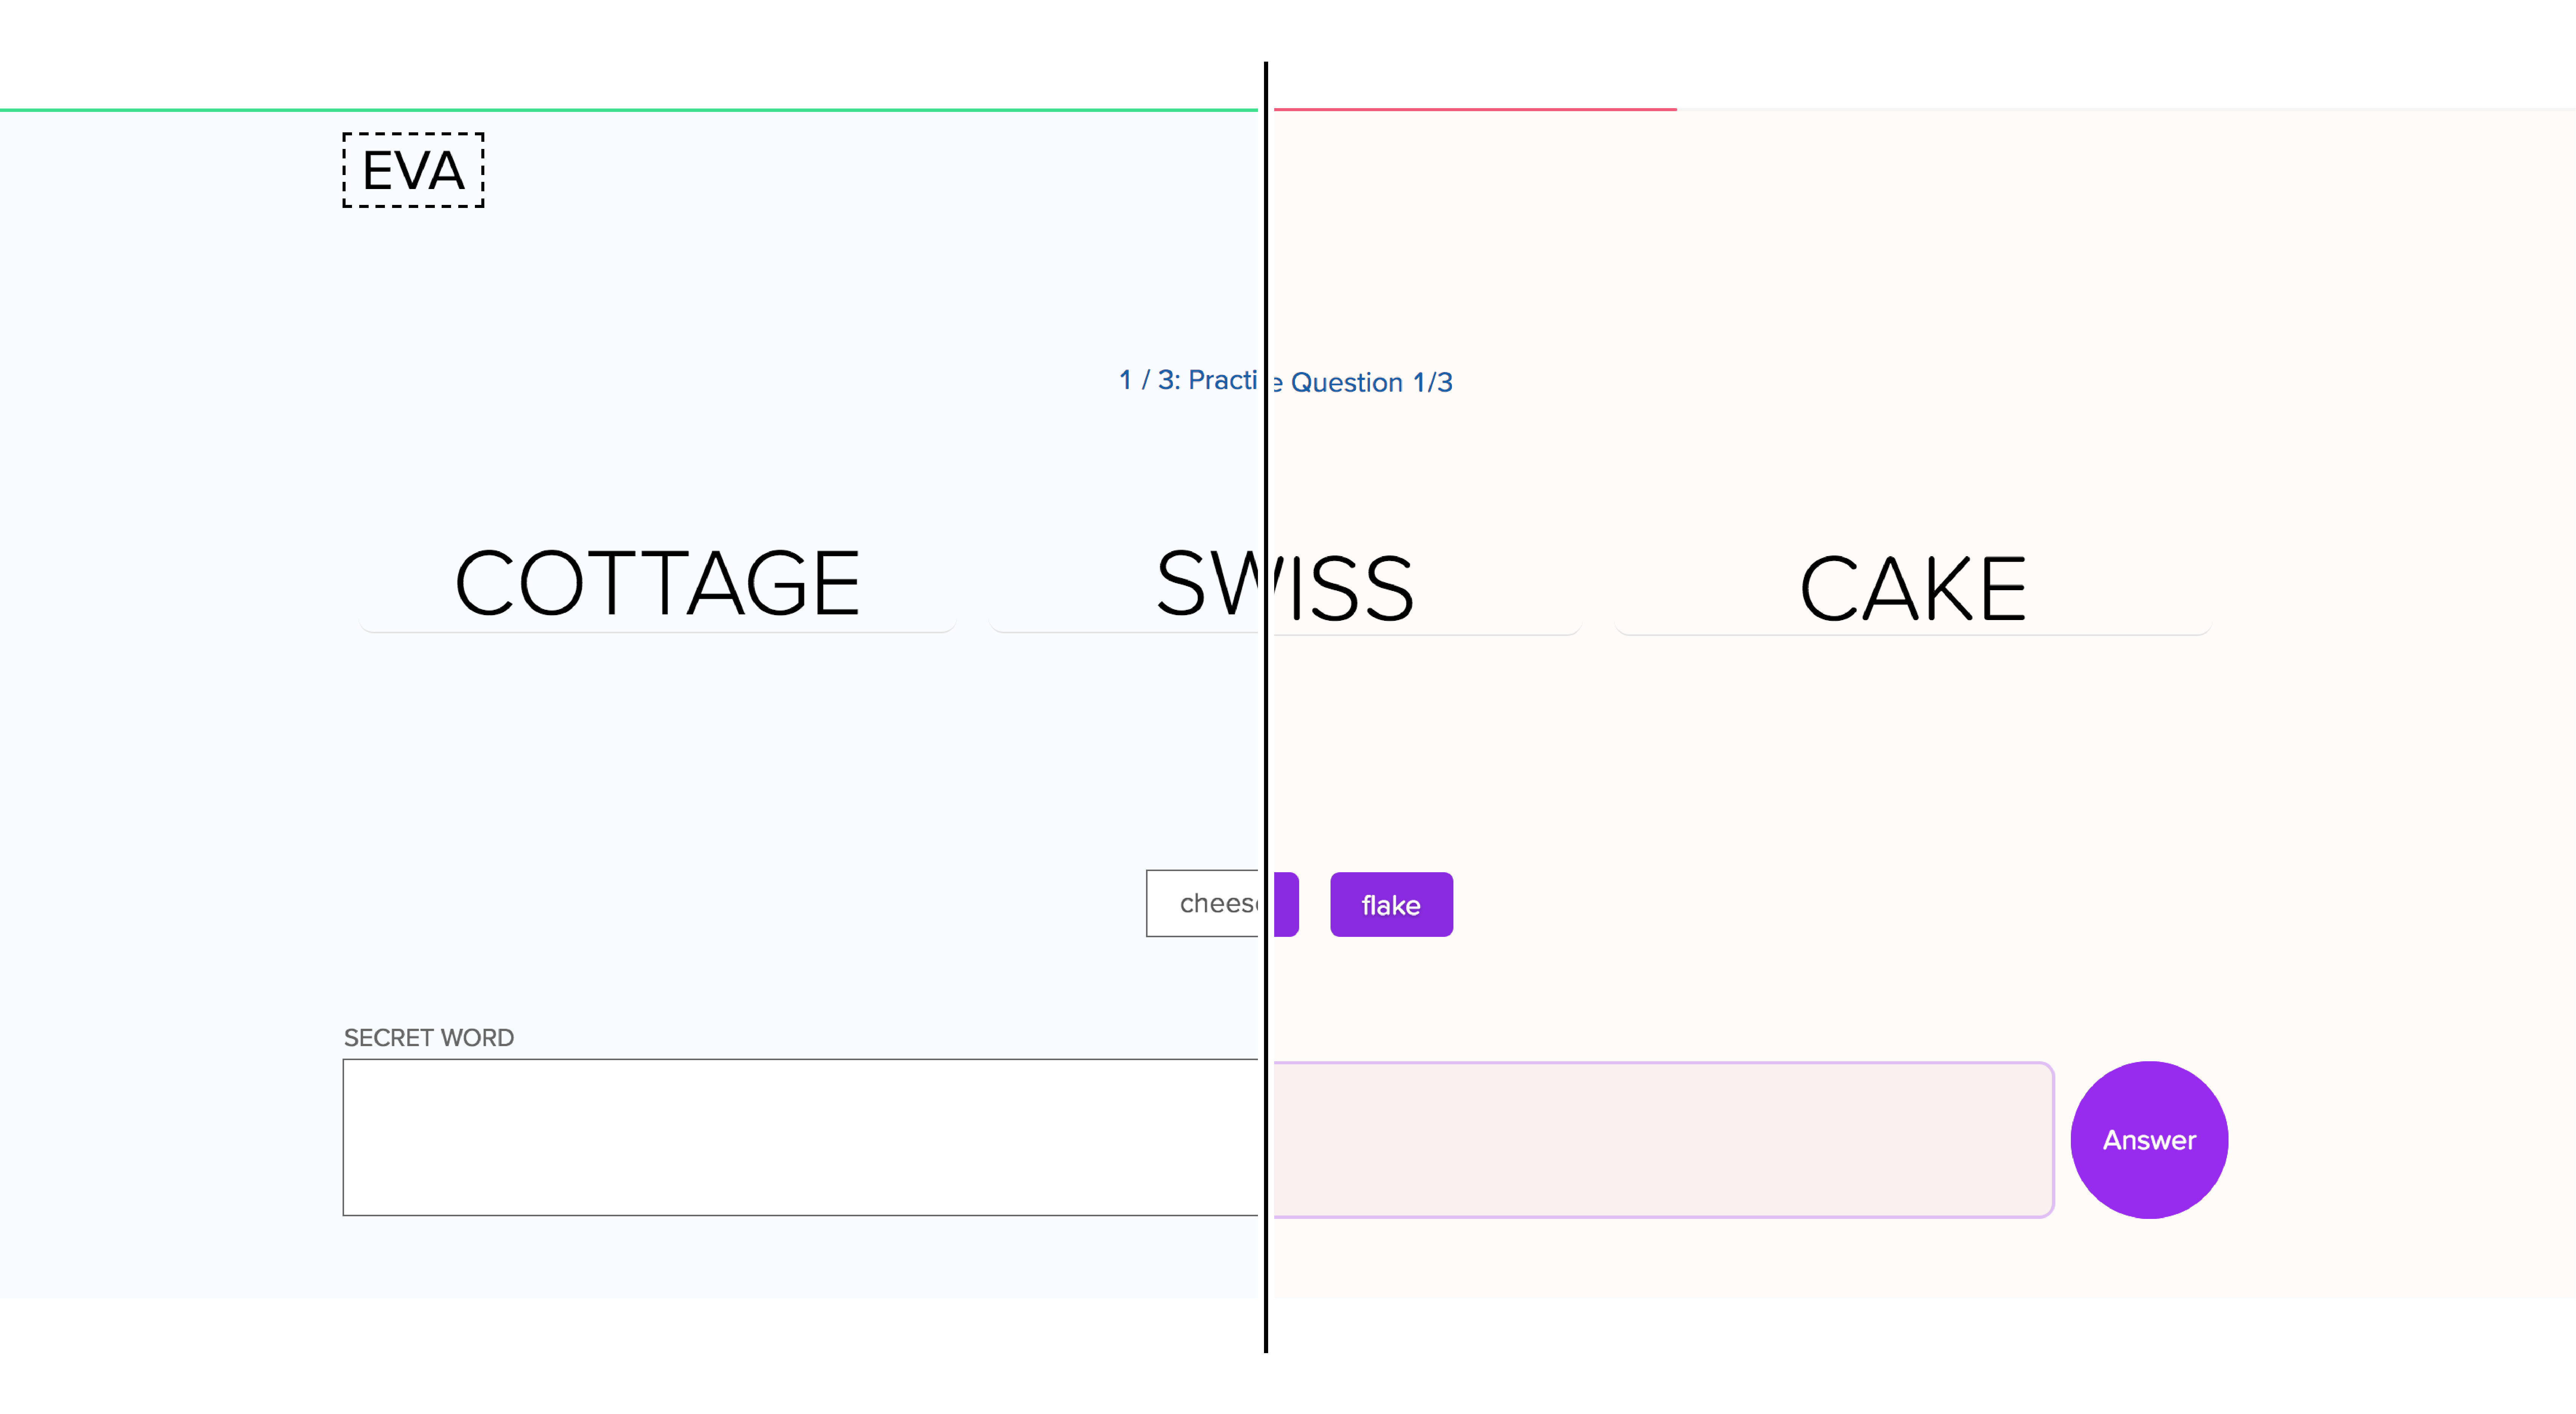
\includegraphics[width=0.7\linewidth]{graphics/creativity-versions}
			\caption{Example screen showing both versions of interface during creativity experiment}
			\label{fig:creativity-versions}
		\end{figure}
	
		After 3 practice tasks, participant clicks on "Start Experiment" before solving 20 items defined in the set. An example preview of both interface screens with the three stimulus words and an input for the answer is displayed in figure \ref{fig:creativity-versions} 
		
		Upon appearance of each word-set a timer starts tracking the time to enter a word.
		Stimulus words appear with a 200ms delay from timer start and 50ms delay between each word appearing. The appearance animation takes 300ms. All items are completely visible at 600ms mark, with the first word in the left-to-right direction completely visible and static at 500ms after timer start. 500ms can be discounted from the time it takes to solve a problem (Effectively participants have 29.5 seconds to solve a problem).
		
		\subparagraph{Appearance of Hints}
		
		Each word-set has a 30 second limit to solve a problem. After time is expired a block with 2 hint words \ref{fig:hint-buttons} appear. One of which is the correct solution to the problem, another is a false solution. It is semantically clear which solution is correct, upon reading it the participant is expected to experience the "aha!" effect mentioned in \cite[p.634]{Bowden} with a reference to previous research. Choosing the wrong answer, once the time expires can be a hint that the participant is not paying attention.
		
		After hints appear, the problem is not any more counted as solved by the participant. 
		
		\textit{Hints appearance can be delayed.} Due to a person requiring time to type the answer on a keyboard it is assumed the answer is known once the first letter of the word is written in the field. There is a 3000ms grace delay to type each additional character. Grace delay accounts for typing speed and is deemed sufficient for most persons. Erasing a character is considered as typing (and resets the counter) unless the first letter of the input is erased. Once the delay is passed or the first letter erased the hints appear and the problem is marked as unsolved. Time of the first letter being typed is considered an objective point of time that a participant figures out the answer to the problem. The time of first letter is always within 30 seconds of appearance of the word-set.
		
		\begin{figure}
			\centering
			
\includegraphics[width=0.3\linewidth]{graphics/Hint-buttons}
			\caption{Hints after time allowed for solving a problem is elapsed}
			\label{fig:hint-buttons}
		\end{figure}
		
		
		Once all items are solved they are directed to the next page of the interface.
				
		\paragraph{Activity logging} \textit{Experiment 2} activity is specified based upon generalized logging of activity in e-learning described in \ref{sec:activitylog}
		
		A generic action emitter triggers an action when either of the following happens:
		
		\begin{itemize}
			\item Click on button to start practice
			\item Click on button to start live experiment
			\item Event when word set appears on screen
			\item Event when word set is guessed correctly
			\item Event when word set is guessed incorrectly
			\item Event when word set has expired (hint words appear)
		\end{itemize}
	
		Each event object contains system status information and context information about current words visible.

		\paragraph{Performance variables} \label{sec:creativity-parameters}
		
		\begin{enumerate}
			\item Aggregated solving speed: seconds taken to solve a problem on average
			\item Non-aggregated solving speed: seconds taken to solve each problem
			\item Idea generation rate: how many attempts (including false ones) are taken within the time limit on average
			\item Success rate: Number of problems solved successfully
			\item Frustration/Negative-attention: Amount of false choices after \textit{Hint Word} suggestion appears as ratio to Hint Word suggestion answers.
		\end{enumerate}
	
		\toDo{elaborate about the measures and reasoning behind them}


	\subsection{Means of emotional self-evaluation} \label{sec:selfeval}
	
	

% \todo[inline, size=\tiny]{'Valence and Arousal evaluation techniques'}


	
	\toDo{Describe Valence and Arousal evaluation methods}  \cite{Harley2016}
	
	SAM , AS, Affect Grid \cite{Russell1989} (the same guy who created the circumplex model 9 years prior), AffectButton \cite{Broekens}
	
	Due to effort constraints of the participants it is important to achieve a intuitive, quick, yet accurate reading of their emotions. In the context of this study self-evaluation is a means to validate results, of Hypothesis 1. I rely on the SAM (Self-Assessment Manikin) method \cite{Bradley1994} to quickly allow users to assess their emotions on a dual 9 point scale. \ref{fig:sam}
	
\begin{figure}
	\centering
	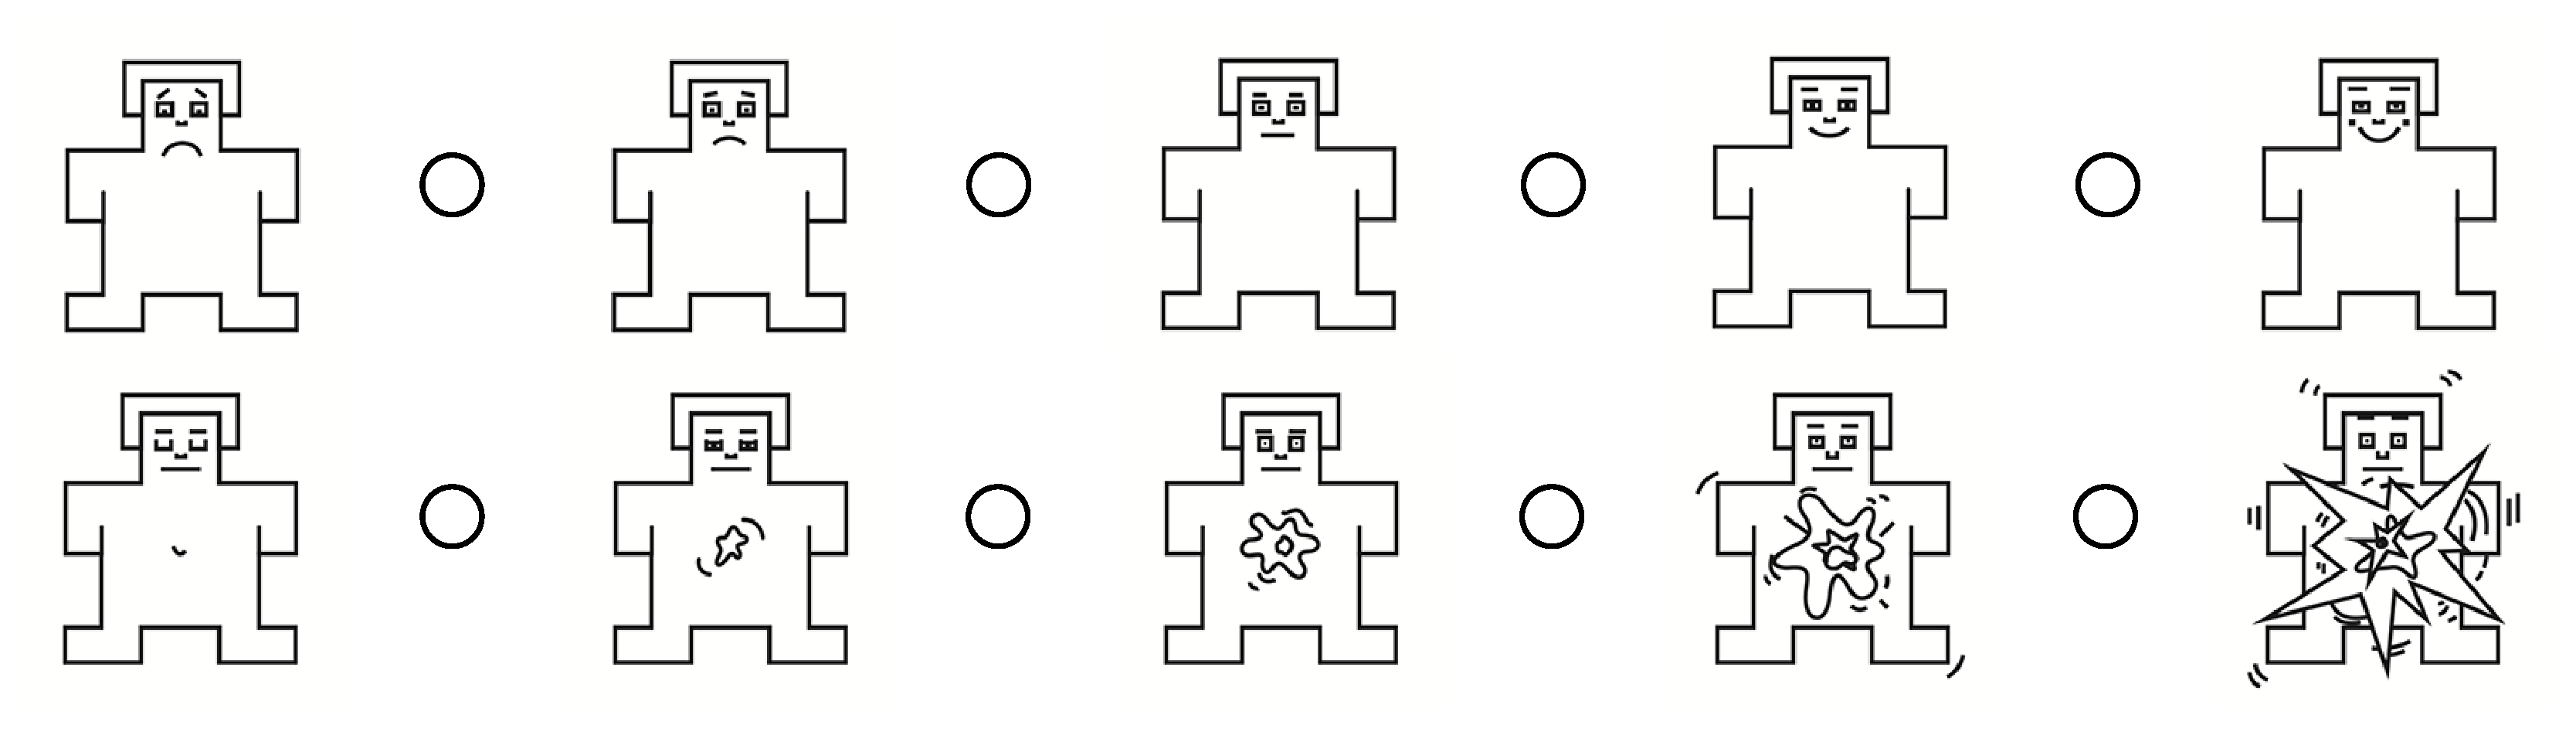
\includegraphics[width=0.7\linewidth]{graphics/SAM}
	\caption{Self-Assessment Manikin. Valence and arousal values}
	\label{fig:sam}
\end{figure}
	
	\subsection{Demographic data and supplemental information} \label{sec:demographics}
	
	As final step of the study each participant fills out a demographics questionnaire to add context data and help with analysis. There are 4 questions:
	
	\begin{enumerate}
		\item Gender \\ \ [Male / Female]
		\item Age \\ \ [18-24 / 25-29 / 30-34 / 35 - 44 / 45 + ]
		\item Is English your native language? \\ \ [yes / no]
		\item What is your level of English knowledge? \\ \
			[Beginner  / Intermediate / Advanced / Fluent]
		\item Occupation: \\ \ [High school student / Undergraduate Student / Graduate Student / Doctorate / Professional or Working]
		\item Email (optional)
	\end{enumerate}

	Gender (Question 1) allows to uncover difference in performance or response due to gender. Possible disparities are expected to be observed as described in \ref{sec:preconditioning}

	The age groups (Question 2) are taken in accordance with suggestions provided by the Standard International Age Classifications \cite{UN1982} with slight modifications to exclude ages below 18.
	
	%Ages above 44 could potentially skew results due to factors not considered by present study. Primary focus audience lies between ages of 18 and 34.
	
	Native speakers (Question 3) might potentially score higher on the creativity task due to cultural influence of using colloquial expressions. This assumption is challenged during data analysis in section \ref{sec:data-validity}
	
	(Question 4) is used to validate the requirement of at least an "advanced" proficiency in English. Participant choosing anything lower could suggest either invalid data or problems with the creativity task due to language issues. In this case participant is considered for removal. \todo{evaluate this claim}
	
	Occupation is inquired for additional context into the participant.
	
	Final "email" field allows the user to enter their email address for participation in the raffle and complies with the motivational promise at the beginning of the experiment.

	\subsection{E-learning activity logging} \label{sec:activitylog}
	%To assess performance of subjects several measurements are taken during the test, these differentiate between the 2 experiments.
	
	Each participant is defined as a \textit{user}. Each user is assigned a session for each new started experiment. 
	
	To assess the performance of participants continuous measurements are taken during a session of the experiment. A general approach is an event-based system where each \textbf{action} from the \textit{user} or the \textit{system} is emitted to the database. A differentiation is established between a "click" action that is initiated by the user and an "event" action that is initiated by the system environment.
	
	For correct attribution at the moment when action is emitted it contains: 
	\begin{itemize}
		\item userID, sessionID, timestamp (unique key)
		\item name of active screen
		\item type of action (\textit{event} or \textit{click})
		\item context information such as global system state and dependent values of current active screen
	\end{itemize}

	Finally, for system actions (events) \textbf{name of event} is provided. For user actions (clicks) a target of the click is provided.
	
	%A session is defined on the scope of single e-learning module and contains user metadata as well as emotional state of the learner.

	

		
		\paragraph{Technical implementation}
		
		Upon requesting the page a user-token is generated and assigned to each participant. This token is saved as a cookie for future reference and visitor matching. Only one successful experiment is allowed per participant due to 
		Each experiment further contains a session object with its attributes. 
		
		"[location]\_[action]\_[result]"
		
		\toDo{[TODO:] describe how tracking is implemented, storage and analysis for current study}
		
		Action tracking is managed by a dedicated module that communicates with the database storage API. Each event sent to the Database is complemented with a timestamp and user data. An action object with usual fields is described in listing \ref{lst:db_object}


	\begin{listing}[H]
		\begin{minted}{json}
			{
			"first": "second1"
			}
		\end{minted}
		\caption{Database Object Fields}
		\label{lst:db_object}
	\end{listing}

\toDo{specify object}

		
		\paragraph{xAPI adaptation} - 
		
		\toDo{[Optional:] explore adaptability and possible constraints}

\section{Study implementation}

\paragraph{Participant sourcing} 
This study includes participants attained through multiple sources:
\begin{itemize}
	\item{Local university:} On-site supervised experiments were conducted on a limited scale to facilitate a clean sample of participants and uncover problems during the study
	
	\item{Local workplace:} On-site semi-supervised experiments are conducted on a limited scale in Berlin area in Germany to facilitate a more diverse sample while keeping controlled environment conditions, similar to university experiments.
	
	\item{Social media:} Remote participants are invited to participate in unsupervised experiments on their own. Channels such as social media, interest groups and university mailing lists are used.
	
	\item{Mechanical turk:} MTurk is one of popuar web services to source participants. Previous research has shown that it can be considered a reliable platform for conducting objective studies. MTurk participants receive monetary compensation for participation \cite{Buhrmester2011a}. Mturk participants are excluded from motivation with a chance on winning a voucher prize (they do not see the field and information box about it), instead regular participant reward through MTurk is used.
	
\end{itemize}

Local and social media experiments provided additional motivation of participation with the promise of a chance to win a 20 Euro Amazon-voucher.

\subsection{Technical implementation} \label{sec:study_technical_implementation}
At the base of current implementation is the requirement to run the study in a browser on a personal computer. 

As the study is done in the field and participants are not supervised I introduce additional checks to ensure that only one session can be completed per one participant. Upon visiting the first page the user retains several cookies that identify them later in the data and during subsequent visits: \textit{userID, sessionID}. UserID is persisted across visits, while sessionID is generated each time the page is loaded and consists of `userID+timestamp`. Once the participant finishes the experiment the session is marked as finished with a cookie

\paragraph{Theme propagation} React.js is selected as a library of choice due to it's favorable characteristics to creating an environment that supports 2 themes and global settings in a scalable way. React's unidirectional data flow allows clear behavior path between application data and visual representation. In particular, it becomes possible to adjust the theme of the interface and propagate in-place an alternative style and visual rules throughout the application without losing current state. Additional benefits of this approach are discussed in section \ref{sec:further-research} in the context of an emotionally aware interface.

\begin{figure}
	\centering
	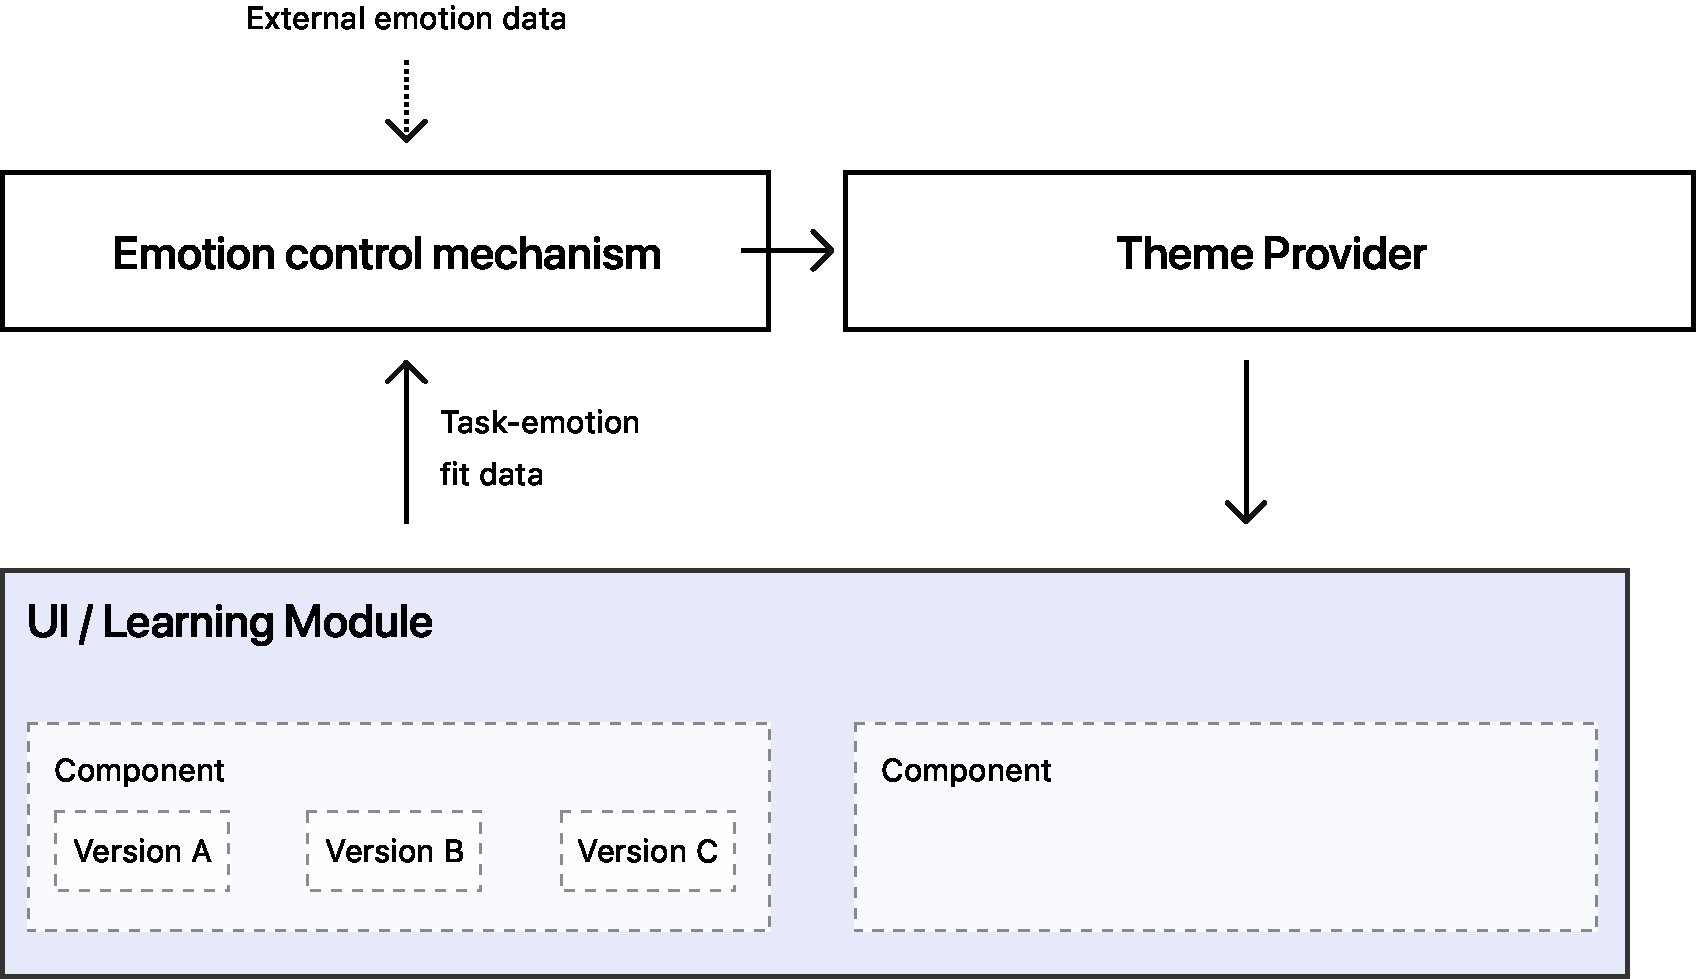
\includegraphics[width=1\linewidth]{graphics/App-Architecture}
	\caption{Component based architecture with emotion control mechanism}
	\label{fig:app-architecture}
\end{figure}

Current implementation contains a minimal proof-of-concept of a way to enable e-learning interfaces to be complemented with emotional data. 

As described in section \ref{sec:research}, research made by \cite{Haaranen2015} puts forth the need to acknowledge current learning context, when deciding on an appropriate emotional-interface response. 
Some emotional-design features may fit best an e-learning module than others.
For example creative tasks might be supported with a warm-colored interface and providing strong degree of control to the user to play around with elements on the screen. 
And analytical tasks might require more concentrated thinking, they might profit from absence of additional distractions, such as images or not directly relevant text. "Seductive details" might cause the learner to concentrate on the wrong content, as proposed by the distraction hypothesis (Harp \& Mayer, 1998) and revisited in \cite{Chang2014}.
Furthermore a distinction can be drawn by learning topic - serious topics can require stricter presentation rules, than entertaining e-learning content.

With the architecture illustrated in Figure \ref{fig:app-architecture}) it is possible to develop an interface that responds to emotional and task contexts with an appropriate interface. A split between presentation layer - UI/Learning Modules, and an "Emotion control mechanism" as well as a "Theme Provider" layer orchestrating UI-level decisions on a global level allows to adjust visual presentation on the fly and from screen to screen.

Learning Modules submit task-emotion fit data to the emotion control layer when each module loads. The emotion control layer then decides on the correct presentation fit which it then passes to the Theme Provider. Additional data about the users emotions can be submitted via self-reporting or through ambient and body-sensors. For the purpose of the study current implementation does not take into account user's self reported emotional affect to adjust the theme. This implementation assigns a theme version at load time and keeps it constant over the course of the experiment.

\section{Results}

	\subsection{Collected data}
	
	Overall one hundred and five \textbf{105} respondents have completed the experiment. Among these 58 (55.2\%) people have been acquired through Amazon Mechanical Turk service, while 47 (44,8\%) have been recruited through social platforms, and local/university.
	
	\paragraph{Population distribution}
	
	In sum forty one (39\%) female participants and sixty four (61\%) male participants finished an experiment session (Table \ref{tbl:gender-distribution}).
	 
	Across five age groups, 11 (10.5\%) participants selected 18 - 24, 34 (32.4\%) are between 25 - 29  years old, 28 (26.7\%) between 30 - 34, 20 (19\%) between 35 - 44, and 12 (11.4\%) are 45 years old or older.
	
	Most popular occupation group is a "Professional" with 65 (61.9 \%) participants reporting it, 17 (16.2\%) in undergraduate studies, 16 (15.2\%) in graduate degree program, 2 (1.9\%) doing a doctorate, as well as 5 (4.8\%) respondents in high school at the moment of participation.
	
\begin{table}[h!]
	\centering
	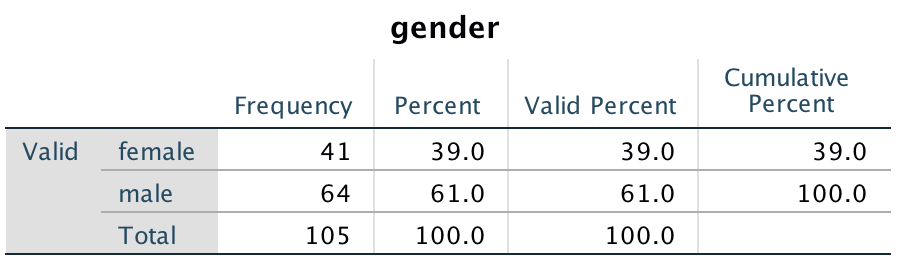
\includegraphics[width=0.7\linewidth]{graphics/Gender-distribution}
	\caption{Distribution of participants by gender}
	\label{tbl:gender-distribution}
\end{table}
	
	\paragraph{Affect levels} Participants rated their mood a total of 3 times, with the first rating making a baseline before testing begins. Valence and arousal values are rated on a 9 point scale with "1" being the lowest rating and "9" - the highest. Table \ref{tbl:distributionOfAffect} shows the affect ratings per preconditioning group. Post Task values include both theme versions in this table. On average participants began with a slightly positive valence (mean 6.08, SE 1.36) and a slightly low level of arousal (mean 3.78, SE 1.8). \toDo{is there a difference Between theme version groups?}
	
	\begin{table}[h!]
	\begin{center}
				
		\begin{tabular}{|c|c|c|c|c|}
			\hline 
			& \multicolumn{3}{c|}{Rating} &  \\ 
			\hline 
			Preconditioning & Initial (1) & Pre Task (2) & Post Task (3) & Observations \\ 
			\hline 
			& \multicolumn{3}{|c|}{Arousal} &  \\ 
			\hline 
			Angry (0) & 3.83 (1.83) & 5.09 (2.15) & 5.04 (1.9) & 23 \\ 
			\hline 
			Happy (1) & 3.72 (1.99) & 4.84 (2.08) & 4.75 (1.95) & 32 \\ 
			\hline 
			Sad (2) & 3.82 (2.08) & 3.95 (1.81) & 4.45 (2.11) & 22 \\ 
			\hline 
			Calm (3) & 4.00 (1.68) & 3.46 (1.53) & 4.54 (1.97) & 28 \\ 
			\hline 
			& \multicolumn{3}{|c|}{Valence} &  \\ 
			\hline 
			Angry (0) & 6.17 (1.19) & 2.39 (1.41) & 5.57 (2.00) & 23 \\ 
			\hline 
			Happy (1) & 5.81 (1.42) & 6.12 (1.39) & 5.00 (2.02) & 32 \\ 
			\hline 
			Sad (2) & 6.41 (1.44) & 4.18 (1.50) & 5.59 (1.56) & 22 \\ 
			\hline 
			Calm (3) & 6.29 (1.36) & 6.07 (1.41) & 5.75 (2.08) & 28 \\ 
			\hline 
		\end{tabular}
	\end{center}
	\caption{Mean (and Standard Error) for each preconditioning}
	\label{tbl:distributionOfAffect}
	\end{table} 
	

	\paragraph{Distribution by english knowledge} 
	
%	\toDo{Describe data preparation, how many people participated, demographics data, distributions.}
	
%	\toDo{Show general statistical data}
	
	\subsection{Data Preparation}
	
	\paragraph{Unique participants} First, a test is made whether all completed experiment sessions are done by a unique user to avoid interference, due to exposure to study in a previous run. Multiple participation shall be excluded, with only the first session being valid under this study design. An SQL query (\ref{itm:sql_check_single_session_per_user}) confirmed, that no participant finished the study multiple times.
	
	\toDo{from events to calculations}
	
	Initial events-based data is transformed into metrics for each participant as displayed in Figure (\ref{fig:participant_attributes}). Prefix "E1" prefix represents Experiment1 - Memory test, and Prefix "E2" represents Experiment2.

\begin{table}
	\begin{center}
		\begin{tabular}{|c|c|c|c|}
			\hline
			\multicolumn{4}{|c|}{Participant Attributes} \\ 
			\hline 
			source & preconditioning & theme version & age \\ 
			\hline 
			gender & education & englishlevel & native \\ 
			\hline 
			arousal preprecond & arousal pre & arousal post &  \\ 
			\hline 
			valence preprecond & valence pre & valence post &  \\ 
			\hline 
			e1 total duration (sec) & e1 pairs opened & e1 false guesses & e1 opens/minute \\ 
			\hline 
			e1 inactive clicks & e1 first miss &  &  \\ 
			\hline 
			e2 avg time/word & e2 time left [word.*]  & e2 idea rate & e2 correct guesses \\
			\hline
			e2 sum bad hint-clicks & e2 neg attention ratio & & \\
			\hline
		\end{tabular} 
	\end{center}
\caption{Participant attributes}
\label{fig:participant_attributes}
\end{table}

	\paragraph{Defining emotion quadrants}
	
	Valence and arousal values are transformed into quadrants with the split in both axes at the value 5.
%quadrant preprecond & quadrant pre & quadrant post &  \\ 


	
	\paragraph{E1 adjusted metrics}
	
	Due to differences in the theme versions the delay for after opening a pair before then next card can be clicked is different. 750ms compared to 1200ms. This delay can cause people to wait longer than they want between opening pairs.
	
	A similar delay of 450ms can be caused between opening first and second card due to animation in theme version "1" which has a delay of 600ms with the image clearly seen after 450ms.
	
	Therefore, I adjust the metrics that are not directly comparable otherwise for participants with theme version 1. Those metrics include the ones that are dependent on time.
	
	\begin{itemize}
		\item e1-total-duration-seconds => e1-total-duration-seconds-adjusted
		\item e1-opens-per-minute => e1-opens-per-minute-adjusted
	\end{itemize}

	\toDo{check if there is a difference of card1 to card2 click delay between versions}
	
	

	
	
	
	\subsection{Validity assumptions} \label{sec:data-validity}
	
		\paragraph{Native speakers} 
		\textbf{H\textsuperscript{0}:}  Native speakers (Question 3) do not score differently on the creativity task due to cultural influence 
		
		\paragraph{Females} 
		\textbf{H\textsuperscript{0}:} Female reaction to Q2 Preconditioning is not different than male
		
		\paragraph{Preconditioning effectiveness}: analyze effect of different precond as a relative and as an absolute for resulting emotional values
	
	
	\subsection{Analysis}
	
	\subsubsection{Hypothesis 1}
	
		First, I check for irregularities with the data and outliers.
	
		\paragraph{Cleaning data}
		
		\begin{figure}
			\centering
			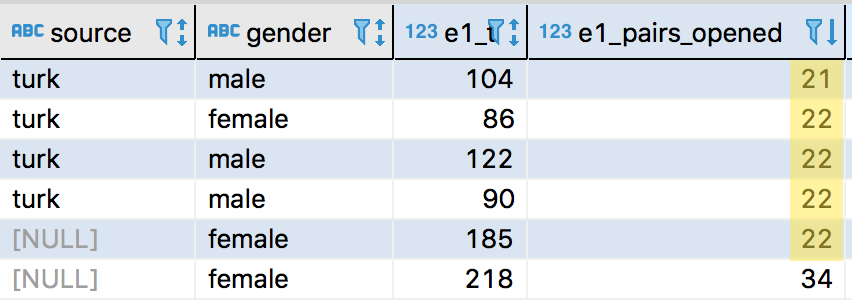
\includegraphics[width=0.7\linewidth]{graphics/MemoryOutlier1}
			\caption{Memory outliers}
			\label{fig:memoryoutlier1}
		\end{figure}
		
		\begin{figure}
			\centering
			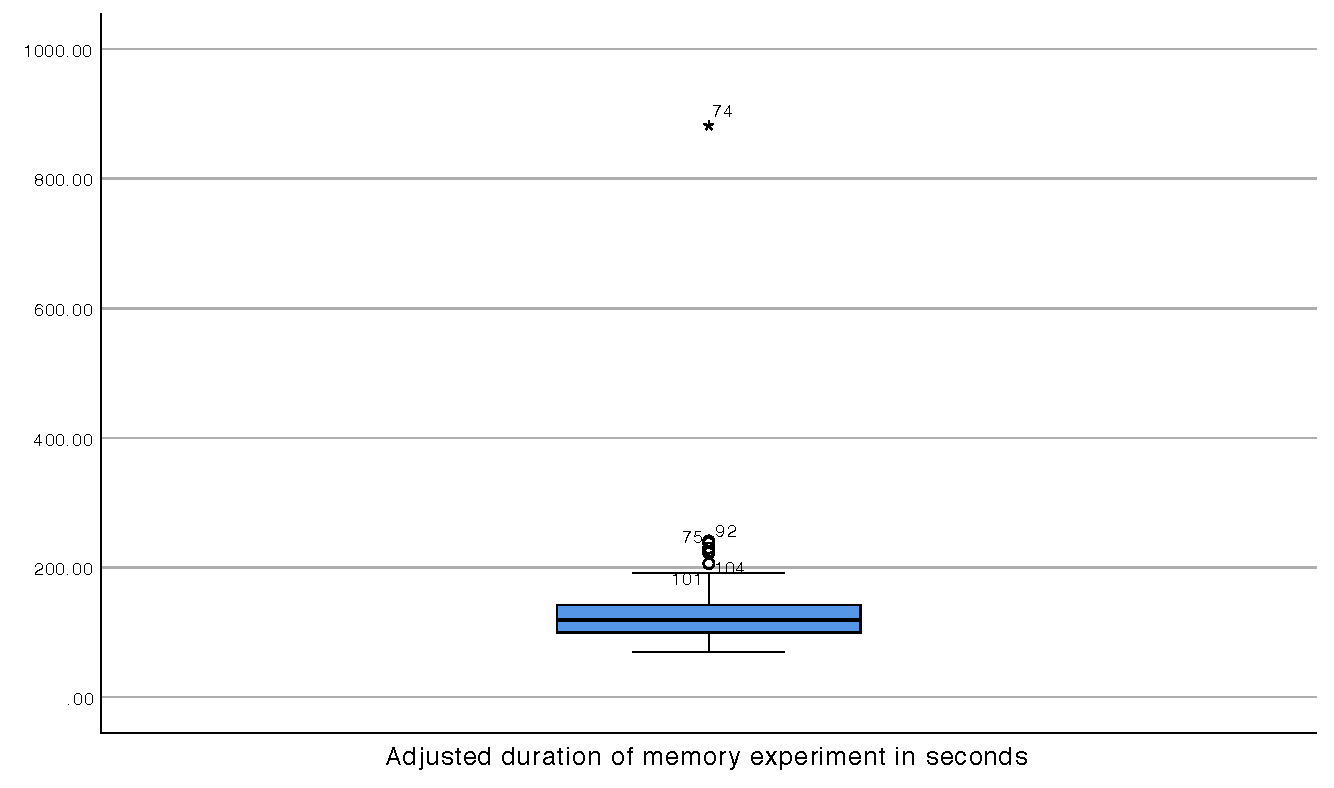
\includegraphics[width=0.7\linewidth]{graphics/memoryOutlier2}
			\caption{Memory duration outliers }
			\label{fig:memoryoutlier2}
		\end{figure}
	
		
	
		Closer look a the data reveals that some users have circumvented the memory game by making a screenshot of the open tiles, or, less probably, having photographic memory. Due to this I exclude these respondents from the memory experiment analysis.
		
		Another outlying data-point is revealed when looking at the overall duration of the memory game in seconds, defined as one of the performance metrics. Respondent \#74 took several times longer than the nearest neighbor.
	
	\subsubsection{Hypothesis 2}
	
	\paragraph{Data selection}
	
	
	
	
\section{Conclusions and Discussion}

	\subsection{Hypothesis 1}
	
	[Note:] H1 should be checked in the context of the whole app
	
	\subsection{Hypothesis 2}
	
	[Note:] H2 should be checked for each task separately
	
	\subsection{Limitations}
	
	\toDo{Show more limitations}
	
	Current assumption of the independence of the emotional axis of the circumplex model of affect can be set into doubt. A neuroscience study \cite{Bestelmeyer2017} analyzing brain signal activation levels suggest an interdependent relationship between pleasure and arousal emotions.
	
	SCHOOL VS COURT conundrum. People can guess court rather than school because it also fits .
	
	EIGHTBALL is USA local
	
	- reported feedback that creativity words are not known to non-natives, frustration and anger during creativity task. Skews results?
	
	Sample size: at 105 participants, although the distributions are healthy it is not possible to factor data by many parameters due to low statistical significance. groups would have each just a few observations.
	
	some subjects reported struggling with the term "valence".

\section{Further research and implications of the study} \label{sec:further-research}

- add dominance to model

- inter-person research of the same person doing the task under different moods. Creativity - not possible.

- Additional benefits of React unidirectional data flow with global theme definition in the context of an emotionally aware interface?

\subsection{Ethical, legal and social implications}

[TODO]

\section{Notes}

\begin{figure}[ht!]
	\centering
	\begin{minipage}{.4\textwidth}
		\centering
		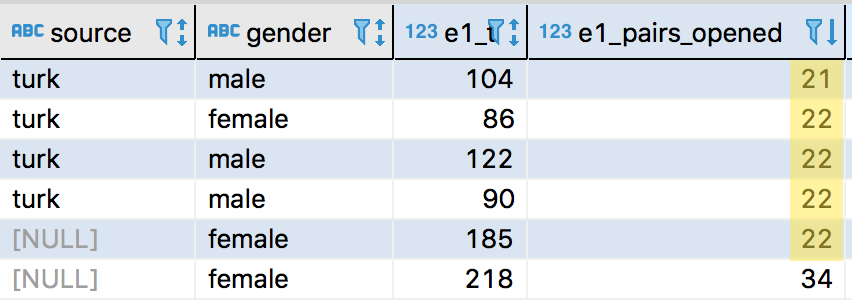
\includegraphics[width=1\linewidth]{graphics/MemoryOutlier1}
		\captionof{figure}{A figure}
		\label{fig:test1}
	\end{minipage}%
	\begin{minipage}{.6\textwidth}
		\centering
		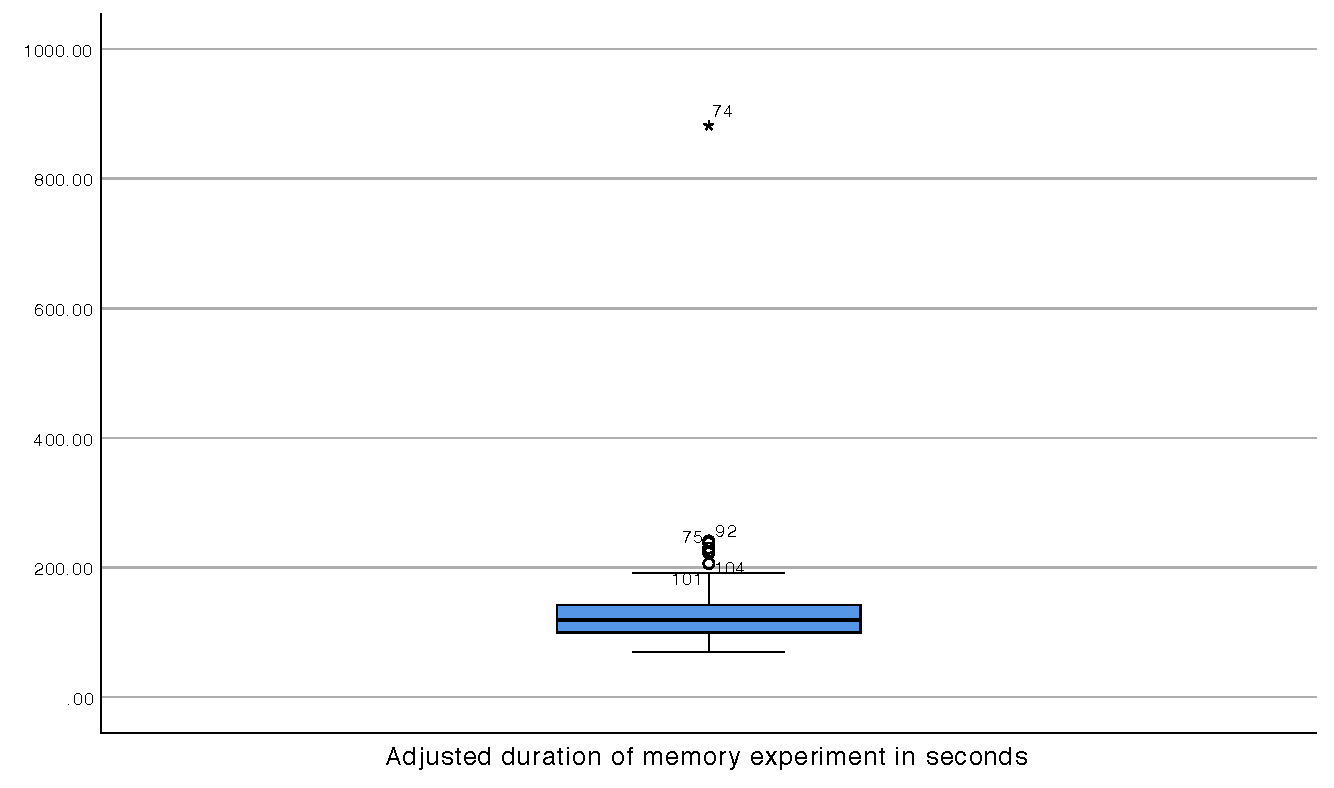
\includegraphics[width=1\linewidth]{graphics/memoryOutlier2}
		\captionof{figure}{Another figure}
		\label{fig:test2}
	\end{minipage}
\end{figure}



